\section{Task: Import JSON Data}
\label{sec:task_import_json}

For information about test dataset please refer to \nameref{sec:test_data}. \\

To execute this task select 'Task'->  'Import JSON Data' in the top menu bar.

\begin{figure}[H]
  \center
    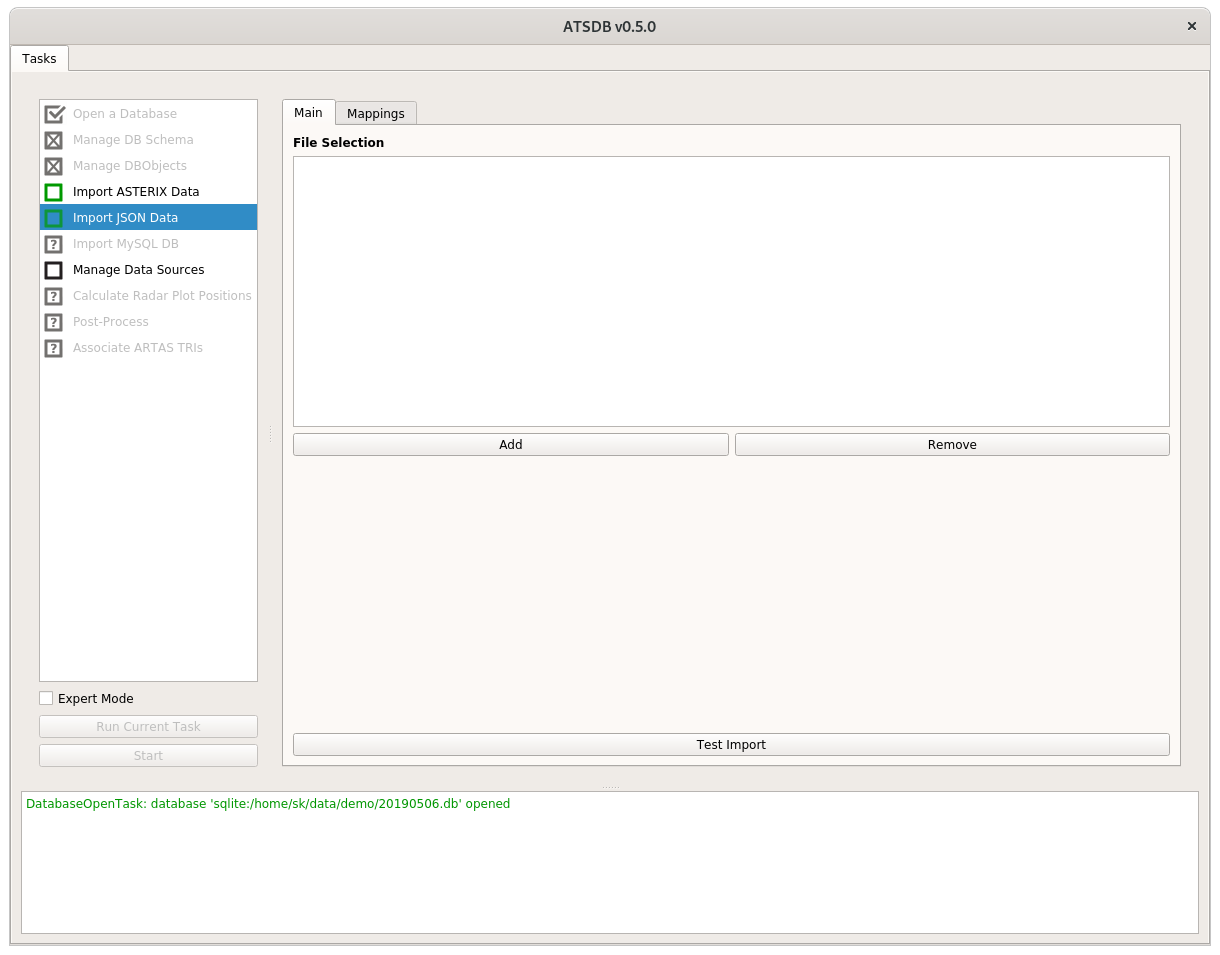
\includegraphics[width=14cm,frame]{../screenshots/import_json_data.png}
  \caption{Import JSON Data task}
\end{figure}

In the 'File Selection' list, a list of available JSON data files is given. Entries can be added using the 'Add' button or removed using the 'Remove' buttons. Please note that either native JSON text files can be imported, or archives containing the same with the following formats: *.zip, *.gz, *.tgz \\

Below, the JSON parsing schema can be selected, the following options exist:
\begin{itemize}  
\item SDDL: Import JSON created by the SDDL v0.2 tool
\item ADSBexchange: Import JSON from the ADSBexchange platform
\item OpenSkyNetwork: Import JSON from the OpenSky Network platform
\end{itemize}

A new schema can be added using the 'Add' button, or an existing removed using the 'Remove' button. \\

Further below, for the selected parsing schema, the list of existing JSON object parsers is shown. Each parser is specialized for a specific DBO, in the shown example of OpenSkyNetwork, only ADSB exists, since no other data is provdided. \\

To inspect or edit a JSON object parser, click on it in the list. This step is not required for parsing.

\begin{figure}[H]
  \hspace*{-1cm}
    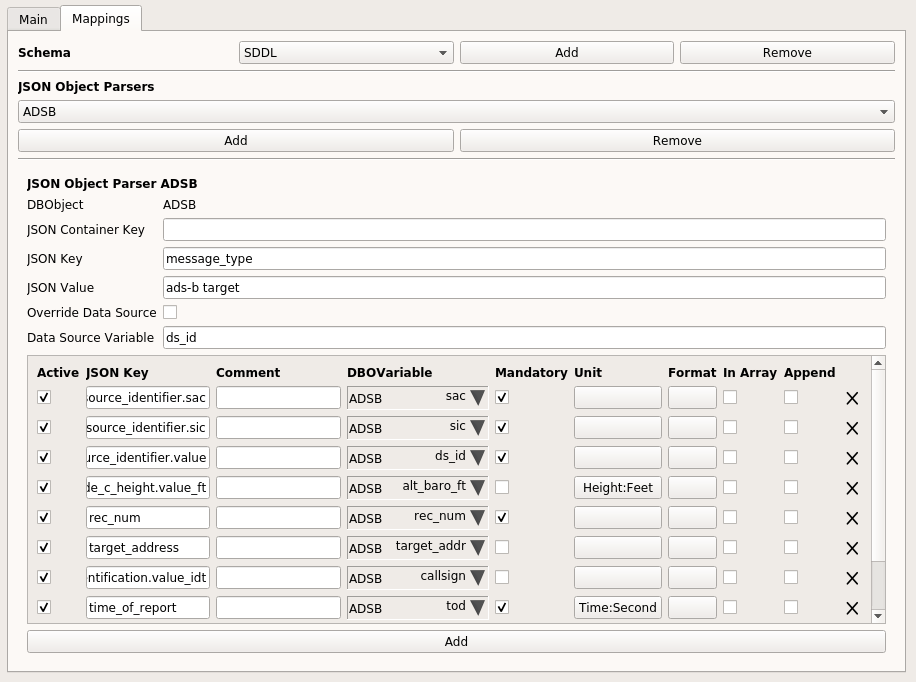
\includegraphics[width=16cm,frame]{../screenshots/import_json_data_object_parser.png}
  \caption{Import JSON Data Object Parser}
\end{figure}

If selected, on the right hand side shows a configuration widget for the selected parser.

\paragraph{JSON Object Parser Configuration}
At the top, a number of configuration options are given:

\begin{itemize}  
\item JSON Container Key: JSON key identifier where nested target reports are stored
\item JSON Key: JSON key identifier for selective parsing
\item JSON Value: JSON value for selective parsing
\item Override Data Source: Checkbox to specify if data source value should be overridden
\item Data Source Variable: Data source variable, for if data source value should be overridden
\end{itemize}


Below list of JSON to DBO variable mappings, with the following options:

\begin{itemize}  
\item Active: Checkbox if mapping should be used for import, mandatory ones must be active
\item JSON key: JSON key identifier
\item DBOVariable: DBO variable that data is mapped to
\item Mandatory: Sets if JSON key/value have to be present, otherwise the JSON object is skipped
\item Unit: Unit of the JSON value
\item Format: Parsing specialization for JSON value
\end{itemize}

A new mapping can be added using the 'Add' button. \\\\

Using the 'Test Import' button, the import function can be tested without inserting the data into the database, the 'Import' imports the selected file with the given options.

During import a status indication will be shown as follows:

\begin{figure}[H]
  \center
    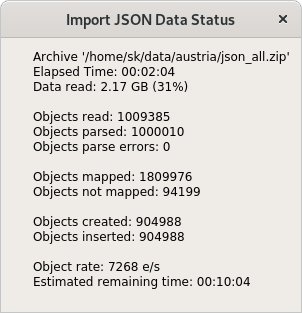
\includegraphics[width=9cm,frame]{../screenshots/json_import_status.png}
  \caption{Import JSON data task status}
\end{figure}

If datasizes can be read from the archive (supported by ZIP but not by GZIP), predictions about the remaining time will be shown.

After import, a confirmation will be shown as follows:

\begin{figure}[H]
  \center
    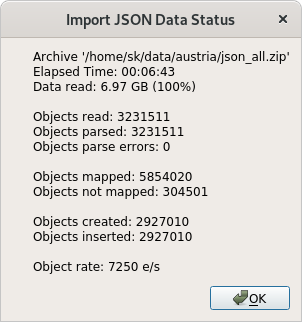
\includegraphics[width=9cm,frame]{../screenshots/json_import_done.png}
  \caption{Import JSON data task done}
\end{figure}

Importing performance strongly depends on CPU performance (multi-threading very beneficial), but a SDDL JSON import of 2.5 million target reports takes about 7 minutes on the author's hardware. \\


\includegraphics[width=0.5cm]{../../data/icons/hint.png} Please note that, since ADSBexchange JSON is not compliant to JSON standard (at least from the used test datasets), parsing errors will be shown and only a small percentage of target reports is imported.
